\chapter{Haemoglobin Fluorescence Self Quenching}\label{app:haemo_self_quench}

\begin{appbox}
	Back to Section~\ref{sect:co2hb:fluo:hb_fluo}\hfill \hyperref[chapter:toc]{Main Table Of Content (TOC)}
\end{appbox}

When measuring the fluorescence of a solution, one might expect to measure more fluorescence signal when increasing the fluorophore concentration. This is however not the case if the fluorophore also absorbs at the wavelength of the re-emitted fluorescent light---a phenomenon known as \emph{self quenching}. The following developments present two simplified models of right-angle and front-face geometry fluorometers to emphasise this latter phenomenon.

\section{Right-Angle Optics}

The geometry of right-angle fluorometers has emerged against classical spectrometers' construction, in order to avoid blinding the detector with the exciting beam\cite{jameson2003}. In a theoretical study however, we are unimpeded by such practical considerations, since an ideal detector can be assumed, sensitive only to the wavelength of the re-emitted light, and not to that of the exciting beam. The right-angle optics can thus be \enquote{unfolded} into a geometry aligning the light source, cuvette, and detector. Such an unfolded spectrofluorometer is depicted in Figure~\ref{annfig:fluo_quenching:fluo_right_spectro} wherein $\Phi_\text{X}(x)$ is the excitation flux at the abscissa $x$ (W.m$^{-2}$), $\Phi_\text{M}(x)$ the re-emitted flux (W.m$^{-2}$), $c$ the solution concentration in fluorophore (M), and $L$ the length of the solution path (m).

\begin{figure}
	\centering
	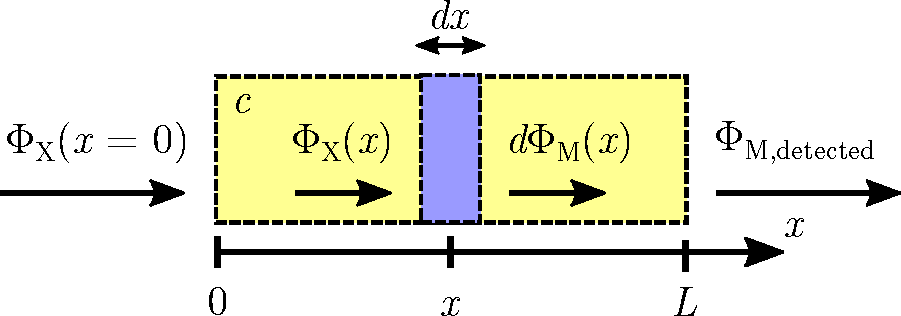
\includegraphics[scale=0.7]{2_appendices/figures/right_angle_scheme.pdf}
	\caption[Right-angle optics scheme.]{Simplified representation of a right-angle optics fluorometer. The input exciting beam---intensity $\Phi_\text{X}(x=0)$---comes from the left of the figure. The output flux to be detected at the emission wavelength exits the cuvette on the right. The solution---concentration in fluorophore $c$---is depicted in yellow. A slice of solution of thickness $dx$ is also represented in light blue. It receives the flux $\Phi_\text{X}(x)$ attenuated by a layer of thickness $x$ of solution. This slice in turns emits fluorescent light in the detector's direction with intensity $d\Phi_\text{M}(x)$. The  light re-emitted by all the cuvette's slices in the 0..$L$ abscissa forms the overall detected light at the detector, $\Phi_\text{M,detected}$.}
	\label{annfig:fluo_quenching:fluo_right_spectro}
\end{figure}

This simple model is considered as a one dimensional problem---along the $x$ axis---and the hypothesis that the solution is purely absorbing---\ie{} without scattering---is also made. This hypothesis holds for diluted lysed blood, which, from being originally translucent but opaque, becomes transparent with haemolysis. Regarding the direction of propagation of the fluorescent re-emitted light, isotropic emission results in half of the emitted light being back-scattered, while half is transmitted in the forward direction (increasing $x$ axis). We can thus write for a small slice of solution
\begin{equation}\label{anneq:fluo_quenching:quantum_yield}
	d\Phi_\text{M}(x)=\sfrac{1}{2} \cdot \eta_\text{Q} \cdot d\Phi_\text{X}(x)
\end{equation}
using the definition of the quantum yield $\eta_\text{Q}$ of a fluorophore\cite{bigio2016}, where $d\Phi_\text{M}(x)$ is the flux emitted by the slice of solution of thickness $dx$ in the detector's direction when absorbing an exciting flux $d\Phi_\text{X}(x)$. Using Beer-Lambert law leads to
\begin{equation}\label{anneq:fluo_quenching:beer_fluo}
	d\Phi_\text{M}(x) = \sfrac{1}{2} \cdot \eta_\text{Q} \cdot \mu_\text{X} \cdot \Phi_\text{X}(x=0) \cdot e^{-x \cdot \mu_\text{X}} \cdot dx
\end{equation}
wherein $\mu_X$ is the attenuation coefficient of the solution at the excitation wavelength (m$^{-1}$), with $\mu_X=c \cdot \varepsilon_\text{X}$, $\varepsilon_\text{X}$ being the molar extinction coefficient of the fluorophore at the excitation wavelength\footnote{Strictly speaking, $\mu_X=c \cdot \varepsilon_\text{X} \cdot \log(10)$, but the $\log(10)$ was omitted for simplification purposes. Similarly, it is assumed that all the forward-propagating light is received at the detector, which is never the case in practice.} (L.mol$^{-1}$.m$^{-1}$). This emitted flux $d\Phi_\text{M}(x)$ is itself absorbed by the solution---of attenuation coefficient $\mu_\text{M}$ at the emission wavelength---before it reaches the detector, following
\begin{equation}
	d\Phi_\text{M,detected}(x) = d\Phi_\text{M}(x) \cdot e^{-(L-x) \cdot \mu_\text{M}}
\end{equation}

To get the total flux at the detector at the emission wavelength, we need to integrate on $L$, leading to:

\begin{equation}
	\begin{split}
		&\Phi_\text{M,detected} = \int_{x=0}^{x=L} d\Phi_\text{M,detected}(x) \\
		&\Phi_\text{M,detected} = \frac{\eta_\text{Q} \cdot \Phi_\text{X}(x=0)}{2} \cdot \frac{\varepsilon_\text{X} }{\varepsilon_X - \varepsilon_\text{M}} \cdot e^{-L\cdot c \cdot \varepsilon_\text{M}} \cdot \left(1-e^{-L\cdot c \cdot (\varepsilon_\text{X} - \varepsilon_\text{M})}\right)
	\end{split}
\end{equation}

Note that in the---highly unlikely---case where $\varepsilon_X = \varepsilon_\text{M}$ the latter equation simply becomes
\begin{equation}
	\Phi_\text{M,detected} = \frac{\eta_\text{Q} \cdot \Phi_\text{X}(x=0)}{2} \cdot \varepsilon_\text{X} \cdot L \cdot c \cdot e^{-L\cdot c \cdot \varepsilon_\text{M}}
\end{equation}


Figure~\ref{annfig:fluo_quenching:fluo_right_curves} depicts several plots of $\Phi_\text{M,detected}$ as a function of the fluorophore concentration $c$ for different values of $\varepsilon_X$ and $\varepsilon_M$, and is useful to understand the self quenching phenomenon that takes place during right-angle haemoglobin fluorescence measurements.

\begin{figure}
	\centering
	\includegraphics{2_appendices/figures/tikz/out/right_angled.pdf}
	\caption[Detected fluorescence intensity in the right-angle optics case.]{Detected fluorescence intensity $\Phi_\text{M,detected}$ as a function of the fluorophore concentration for different $(\varepsilon_\text{X},\varepsilon_\text{M})$ values, taking unitary $\eta_\text{Q}$, $L$ and $\Phi_\text{X}(x=0)$.}
	\label{annfig:fluo_quenching:fluo_right_curves}
\end{figure}

At first, we can notice that in the absence of absorption at the emission wavelength---red curves---increasing the fluorophore concentration above a certain threshold is pointless. Indeed, the re-emitted light---and thus detected light, since all the re-emitted light will be collected without attenuation---becomes limited by the intensity of the exciting beam $\Phi_\text{X}(x=0)$. In this configuration, the collected light is directly proportional to the exciting beam intensity, given that the fluorophore concentration is at least three up to five-fold larger than $(\varepsilon_\text{X} \cdot L)^{-1}$ (first-order exponential decay).

Then, if the fluorophore also absorbs at the emitting wavelength, as is the case for haemo\-globin---green and blue curves---it appears that there is an optimal concentration to measure the highest possible fluorescence intensity, where the fluorescence intensity peaks---typically in the 0.5--3~M range in Figure~\ref{annfig:fluo_quenching:fluo_right_curves} depending on which blue or green curve is taken. The higher the fluorophore absorption at the re-emitted wavelength, the lower the fluorophore concentration should be to maximise $\Phi_\text{M,detected}$, but also the lower the $\Phi_\text{M,detected}$ value will be. This illustrates well the so-called \enquote{self quenching} mechanism.

As a quick application, taking the extinction coefficients of Prahl\cite{prahl1998} for \gls{o2hb} and an optical path length of approximately 1~cm---as is the case in commonly encountered right-angle fluorometers---leads to an optimal fluorophore concentration of 10~{\textmu}M for an excitation at 280~nm and an emission at 326~nm. The measurements related in Section~\ref{sect:co2hb:pulse_carbametry} were performed with $c\approx20$~{\textmu}M, and were thus well targeted, being in the corresponding fluorescence intensity peak (peak over its half-width in the 1--25~{\textmu}M range).

\subsection{Front-Face Optics}

In the case of front-face optics, the geometry depicted in Figure~\ref{annfig:fluo_quenching:fluo_front_spectro} will be considered. It is quite similar to that of Figure~\ref{annfig:fluo_quenching:fluo_right_spectro}, with the exception that the detector is now located on the same side as the exciting beam source.

\begin{figure}
	\centering
	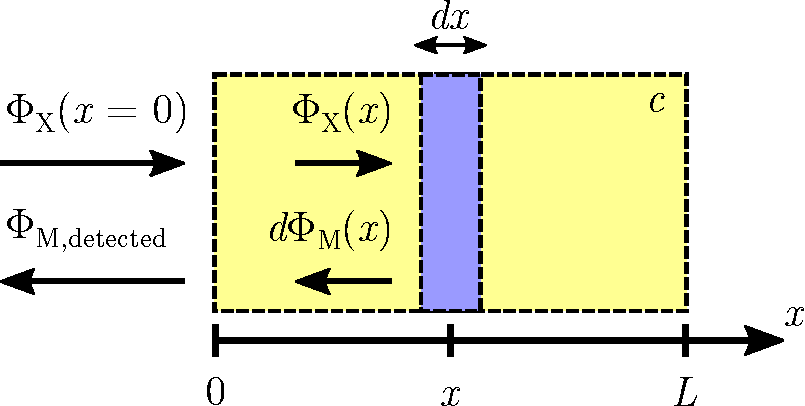
\includegraphics[scale=0.7]{2_appendices/figures/front_face_scheme.pdf}
	\caption[Front-face optics scheme.]{On this variant of Figure \ref{annfig:fluo_quenching:fluo_right_spectro}, the re-emitted light exits the sample from the same side as it enters it. In other words, the detector is located on the same side as the exciting beam (left side of the figure).}
	\label{annfig:fluo_quenching:fluo_front_spectro}
\end{figure}

The same reasoning as in the previous section can be followed, now considering only the part of the emitted light that is backward-propagating towards the detector. Equations~\ref{anneq:fluo_quenching:quantum_yield} and \ref{anneq:fluo_quenching:beer_fluo} still hold, and the re-emitted flux that reaches the detector after partial absorption is
\begin{equation}
	d\Phi_\text{M,detected} = d\Phi_\text{M}(x) \cdot e^{-x \cdot \mu_\text{M}}
\end{equation}

Integrating on the full length of the cuvette yields
\begin{equation}
	\begin{split}
		&\Phi_\text{M,detected} = \int_{x=0}^{x=L} d\Phi_\text{M, detected}(x) \\
		&\Phi_\text{M,detected} = \frac{\eta_\text{Q} \cdot \Phi_\text{X}(x=0)}{2} \cdot \frac{\varepsilon_\text{X} }{\varepsilon_\text{X} + \varepsilon_\text{M}} \cdot (1-e^{-L\cdot c \cdot (\varepsilon_\text{X} + \varepsilon_\text{M})})
	\end{split}
\end{equation}
and the corresponding fluorescence intensity curves are presented in Figure~\ref{annfig:fluo_quenching:fluo_front_curves}. Contrary to the right-angle case, an increase in the fluorophore concentration does not result into a decrease in fluorescence intensity in case of non-null $\varepsilon_\text{M}$---blue and green curves.

One can see that given that \emph{(i)} the solution is sufficiently concentrated, \emph{(ii)} the cuvette is long enough, or \emph{(iii)} the molar absorption coefficients are high enough, the intensity of the fluorescent light measured with such a system is only a function of the $\sfrac{\varepsilon_\text{X}}{\varepsilon_\text{X} + \varepsilon_\text{M}}$ ratio, $\eta_\text{Q}$ and $\Phi_\text{X}(x=0)$. In other words, if the afore-mentioned conditions are fulfilled, the fluorescence measurement only depends on the fluorophore and the fluorometer, but not on the concentration of the former nor on the cuvette's depth. This is because the exciting beam is only probing a superficial layer of the cuvette, and we could even define the value $(c\cdot(\varepsilon_\text{X} + \varepsilon_\text{M}))^{-1}$ as the \emph{characteristic depth} probed by the exciting beam.

\begin{figure}
	\centering
	\includegraphics{2_appendices/figures/tikz/out/front_face.pdf}
	\caption[Detected fluorescence intensity in the front-face optics case.]{Detected fluorescence intensity $\Phi_\text{M,detected}$ as a function of the fluorophore concentration in the case of front-face optics for different $(\varepsilon_\text{X},\varepsilon_\text{M})$ values, taking unitary $\eta_\text{Q}$, $L$ and $\Phi_\text{X}(x=0)$.}
	\label{annfig:fluo_quenching:fluo_front_curves}
\end{figure}

Such calculations are in good agreement with the results presented by Hirsch \textit{et al.}\cite{hirsch1980} when using the haemoglobin extinction coefficients provided by Prahl\cite{prahl1998}. Last detail, with such extinction coefficients and at a physiological haemoglobin concentration (that of blood for instance), the latter characteristic depth is as low as 4.2~{\textmu}m. Probing tissues with fluorescence transcutaneously at the considered wavelengths is thus most certainly unfeasible.

\begin{appbox}
	Back to Section~\ref{sect:co2hb:fluo:hb_fluo}\hfill \hyperref[chapter:toc]{Main Table Of Content (TOC)}
\end{appbox}